\subsection{6 RL 与 OPD 基础设施}\label{rl-and-opd-infrastructure}

MiMo-V2.6 系列将 RL 与 OPD 训练扩展到由智能体 rollout 构成的大规模混合任务批。为支持灵活的智能体 rollout 场景，我们定义了执行模型与轨迹数据结构，并用惩罚模块（Penalty Module）细化学习信号（§6.1）。在大批大小下，我们实现 Harness Pool 来承载多个脚手架并维持高 rollout 并发，实现 Payload Porter 来缓冲数万条携带路由与多模态数据的重型轨迹（§6.2）。我们实现 Sample Mixer，它与动态采样器和部分 rollout 协同，稳定地产出符合指定训练分布的训练批（§6.3）。为稳定高效的 RL 训练，我们在训练引擎与推理引擎之间对齐 MoE 路由与 top-p 采样候选集，同时针对 RL 负载优化这两个引擎（§6.4）。

\subsection{6.1 细粒度学习信号的智能体 RL}\label{agentic-rl-with-fine-grained-learning-signals}

智能体 rollout 跨越多轮与多个对话上下文，而结果奖励只提供粗粒度监督。因此我们采用以智能体为中心的执行模型，并把轨迹数据组织为层次结构。在该层次结构内，可配置的惩罚模块施加损失掩码与优势塑形。它针对模型自身的局部错误，并把基础设施故障排除在训练信号之外。



Agent Loop 我们把 rollout 从以推理为中心的设计转向以智能体为中心的设计：每条序列作为一个 Agent Loop 运行，它拥有环境生命周期、管理自己产生的对话，并按需调用推理引擎。生命周期涵盖建立、交互、奖励评估（例如运行测试用例）与清理。交互期间，loop 暴露一个请求端点，外部智能体通过调用它来驱动 rollout。每段对话同时以字符串前缀和 token 序列两种形式保存。前缀匹配定位到来请求所扩展的那段对话，只对新后缀做分词并送入推理引擎，使其接口保持纯粹的 token 进、token 出。

轨迹层次结构 子智能体、上下文压缩与多种智能体角色会在一次 rollout 内产生并发的对话分支。我们把轨迹数据组织为四级层次：Sample $\to$ Sequence $\to$ Context $\to$ Segment。Sample 是由 Sample Mixer 派发的一条提示（§6.3）。在 GRPO（Shao et al., 2024）这类组内算法中，一个 Sample 派生出一组 Sequence，该组作为整体被接受或拒绝。一个 Sequence 是一次 Agent Loop 执行，可包含多个并发 Context。一个 Context 是一条对话分支，持有一个 Segment 列表；它是前缀匹配、KV 缓存复用与训练数据导出的单位。一个 Segment 是单轮——一条系统或用户消息、一次模型生成，或一个工具结果——只有模型生成的轮次参与损失。

惩罚模块 组内算法把结果奖励均匀分摊到一条序列中所有模型生成的 token 上。在上述层次结构中，功劳很少是均匀的：有些轮次偏离路径或退化，有些失败与模型无关。为把功劳归于应得之处，我们把检测与其对训练的影响分开。Rule 通过手工逻辑或基于模型的裁判来评判一个 segment、context 或 sequence。例如，规则可以捕捉不可归因于模型的基础设施故障、乱码 token 模式、对不可用工具的调用以及重复。Strategy 把一个动作绑定到层次结构的某一层：mask 把命中的内容排除出损失，优势塑形对命中 token 上的优势进行设置、缩放或减去，monitor 只记录指标。复合的 early stop 策略在其规则触发时立即终止 rollout，把结果奖励置零，对触发轮次与更早的轮次施加不同的动作，并掩蔽同级 context。惩罚沿层次结构逐级升级：没有存活模型轮次的 context 被丢弃，没有存活 context 的 sequence 获得零优势，没有存活 sequence 的 sample 被拒绝。训练中实际施加的具体惩罚见 §4.3.3。

\subsection{6.2 Harness Pool 与 Payload Porter：多脚手架的大批大小 RL}\label{harness-pool-and-payload-porter-large-batch-rl-with-multiple-harnesses}

把 RL 训练扩展到大批会提高 rollout 并发度，也提高轨迹数据的内存与通信开销。混合任务批又增加了异质性的一个维度：单个批混合多个脚手架，每个训练样本组绑定到一个脚手架。在执行侧，Harness Pool 把并发的脚手架实例与 Agent Loop 托管在常驻的多租户 actor 池中，脚手架代码库、智能体行为与环境设置各自独立配置。在数据侧，Payload Porter 让 driver 仅凭轻量元数据完成调度。重型 payload 一次性写入分布式存储，并在被消费处打包。多模态 payload 按同样方式拆分为元数据与像素，并采用增量传输与负载均衡编码。




\begin{figure}[htbp]
\centering
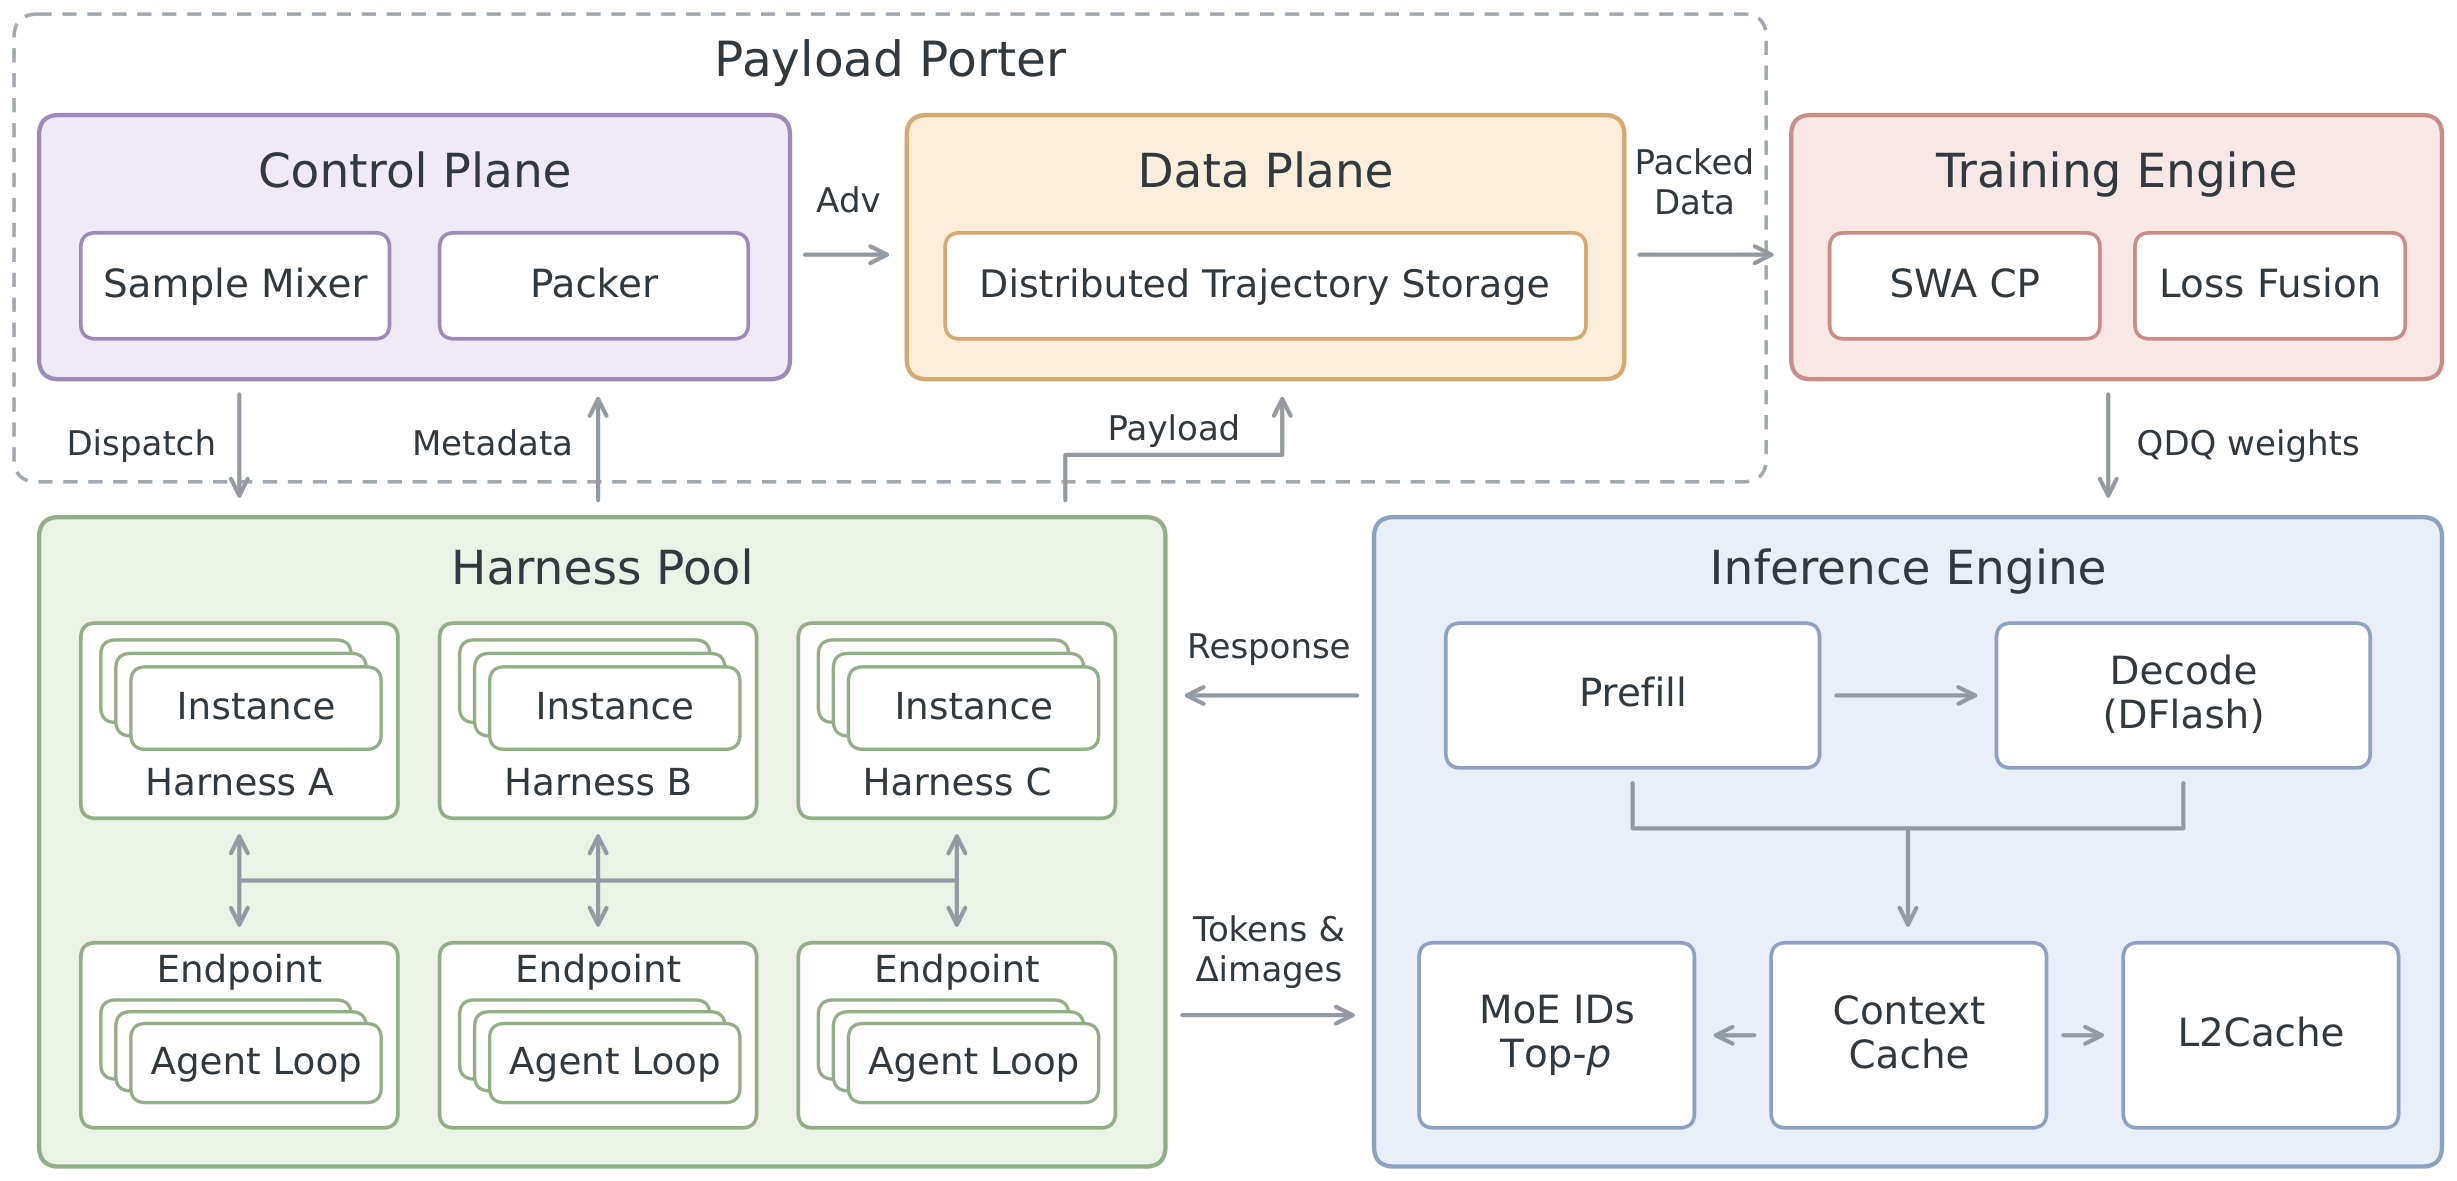
\includegraphics[width=\linewidth]{images_hi/fig14.png}
\caption{RL 基础设施的总体架构。}
\label{fig:14}
\end{figure}

多租户 rollout 执行 我们用 Ray actor（Moritz et al., 2018）在集群上执行智能体脚手架与 Agent Loop。若为每个脚手架实例和 Agent Loop 都分配一个专用 Ray actor，会在 Ray 的全局控制存储（GCS）节点上为每个 actor 占用一个文件描述符，而大批会耗尽 GCS 节点的文件描述符。我们改为运行固定大小的常驻 host actor 池，每个 host 承载许多并发租户——模型侧的 Agent Loop 与环境侧的脚手架实例。每个租户保持自己的轨迹状态，分配按在途实例数做均衡。一个 host 是一个单一进程，其租户共享一个事件循环。模型侧的租户还共享一个请求端点、一个推理代理和一个分词器；环境侧的租户共享一个已导入的脚手架代码库。共享事件循环会让一个阻塞调用拖住所有租户，因此阻塞型工作——环境操作与分词——放在后台线程上运行。这样把进程与服务开销摊销到并发 rollout 上，从而支持更大的并发批，而 actor 数量不会成比例增加。

异构智能体脚手架 我们分别配置脚手架代码库、智能体行为与环境设置，以在单次训练运行中容纳多样的任务。不同数据源可以使用不同的代码库，而智能体配置在同一数据源内随提示不同而变化。每个训练样本组使用统一配置，以便做组内相对优势估计。一个进程只能导入一个脚手架代码库，因此不同代码库运行在各自独立的池中。这些池从固定的 host actor 预算中获得可配置的份额——预算在启动时设定一次，与每步调度的训练数据配比无关。脚手架多样性与 rollout 并发度因此可以在同一个执行框架内扩展。

数据面与控制面分离 扩展后的批必须一次缓冲数万条序列，且每条都很重：除 token id 与对数概率外，还携带 MoE 路由数据、top-p 采样索引与多模态数据。payload 体量随序列数量与长度一同增长，而把所有 payload 汇聚到单个 driver 节点会使批大小受限于该节点的内存。因此我们把数据面与控制面分离，在 rollout 结束时对每条序列做切分：其 payload 一次性写入分布式键值存储（例如 Ray object store 或 TransferQueue（Han et al., 2025）），而 driver 仅凭轻量元数据完成全部调度——标量奖励、各 context 的长度，以及寻址每个 payload 的键。在组结束时，只从存储读取所需字段：accept-time 钩子需要的少数几列。组内评分器在配置后会与 Agent Loop 完全异步地运行——其延迟被隐藏，结果可以滞后——并在返回时改写组奖励。采样器随后仅凭元数据按通过率接受或拒绝该组，钩子则施加长度惩罚、计算组内相对优势并施加优势塑形。逐 token 优势被写回存储；优势全为零的组默认被丢弃。在 OPD 下，奖励评估被教师打分取代：每条轨迹被送往教师服务器，其分数被异步收集到同一个分布式存储中。在批产出时——即每个数据源都贡献了其在批中的份额之后——产出钩子把被接受的序列打包成微批并分配到各个 rank，不触碰任何张量。打包时，每个训练张量并行（TP）组由一个 packer 服务该组内的所有 rank。它从存储中未填充的行里，只取自己的上下文并行（CP）窗口覆盖到的行，并只切出该窗口。结果作为单个只读的内存副本在 TP 组内共享。这避免了 driver 上的全批聚合以及打包期间的稠密填充中间量。



多模态数据 多模态 payload 遵循同样的元数据/payload 拆分，但需要额外小心：随着智能体在多轮中反复截图和读取图像，单条轨迹可能累积数 GB 的此类数据——存储代价高，且随着历史增长重传代价也高。因此在 rollout 期间，Agent Loop 只发送请求之间的多模态增量（§6.4）。训练时，每个图像条目都必须经过视觉编码器。由于编码器在张量并行组内是复制的，而 LLM 主干是分片的，编码先以数据并行方式运行——图像条目在各 rank 间均衡分配，与各序列 token 的落点无关。编码后，嵌入被重分配到持有对应 token 的 rank 上。payload 本身留在分布式键值存储中：负载均衡规划只读取条目元数据，像素只在编码器计算时取用。这在容纳不均衡的多模态负载的同时，限制了冗余的 payload 搬运。
